Jacobson~\cite{j1989} first proposed to design succinct data structures. Under the bit probe model, he showed how to represent an ordinal trees on $n$ nodes using $2n+o(n)$ bits, to support the computation of the first child, the next sibling and the parent of any given node in $O(\lg n)$ time. 
Under the word RAM model with $\Theta(\lg n)$ word size, Clark and Munro~\cite{cm1996} showed how to support these operations in constant time. 
Since then, a lot of work has been done on succinct tree representations, to support more navigational operations in trees, to achieve compression, to provide support for update operations, and so on~\cite{mr1997,bdmr1999,grr2004,jss2007,ly2008,hms2012,fm2014,Navarro:2014:FFS:2620785.2601073}. 
All this work created several different ways of representing trees succinctly, and we refer to the article by Raman and Rao~\cite{rr2013} for a thorough survey.



Among the different approaches of representing trees succinctly, we choose to design a parallel algorithm to construct the most recent work by Navarro and Sadakane~\cite{Navarro:2014:FFS:2620785.2601073}, who used the term {\em fully functional} representation to refer to their work. There are several reasons. 
First, their work is the first that achieves a {\em redundancy} of $O(n/\lg^c n)$ bits for any positive constant $c$. 
In succinct data structures, redundancy is defined to be the difference between the actual space cost of the data structure and the information theoretical lower bound, and this quality is of both theoretical and practical importance. 
While all the work mentioned here has a redundancy of $o(n)$ bits, all but the fully functional representation requires a redundancy of $\Omega(n \lg\lg n / \lg n)$ bits. 
Second, the fully functional representation supports a large number of navigational operations in trees. Only the work in \cite{hms2012,fm2014} supports two more operations. 
Table~\ref{tbl:operations} gives the list of operations supported in constant time by the fully functional representation, in which the first group of operators are navigational operators in trees. 
Finally, the most recent experimental studies on succinct trees~\cite{ACNSalenex10} showed an implementation of the fully function representation indeed uses less space than the existing implementations of other succinct tree representations in most cases, and provides faster support for most operations. Thus it is more suitable for most practical applications. 


\begin{table}[t]
\begin{center}
\begin{tabular} {|p{2.4cm}|p{5.2cm}|} \hline
operator name                             &descriptions        \\ \hline
%$\rmqi(i,j)$ /$RMQi(i,j)$             &Position of the minimum/maximum excess value in $P[i..j]$ \\ \hline
$\child(x,i)$                         & $i$th child of node $x$\\
$\child\_rank(x)$                     & Number of left siblings of node $x$\\
$\degree(x)$                          &Degree of node $x$\\
$\depth(x)$                           & Depth of node $x$\\
$\levelanc(x,i)$                      &Ancestor of node $x$ that is $i$ levels above node $x$ \\
$\subtreesize(x)$                     &Number of nodes in the subtree rooted at node $x$ \\
$\height(x)$                          &Height of the subtree rooted at $x$ \\
$\deepestnode(x)$                     &Deepest node in the subtree rooted at node $x$\\
$\lca(x,y)$                           &Lowest common ancestor of nodes $x$ and $y$ \\
$\lmostleaf(x)$ /$\rmostleaf(x)$      &Leftmost/rightmost leaf of the subtree rooted at node $x$\\
$\leafrank(x)$                        &Number of leaves before node $x$ in preorder\\
$\leafselect(i)$                      &$i$th leaf from left to right\\
$\prerank(x)$ /$\postrank(x)$             &Number of nodes preceding node $x$ in preorder/postorder\\
$\preselect$ /$\postselect(i)$            &$i$th node in preorder/postorder\\       
$\levellmost(i)$ /$\levelrmost(i)$       &Leftmost/rightmost node among all the nodes with depth $i$ \\
$\levelsucc(x)$ /$\levelpred(x)$        &Node immediately to the left/right of node $x$ among nodes with depth $i$\\ \hline
$\access(i)$                           &$P[i]$        \\ 
$\findopen(i)$ /$\findclose(i)$       &The matching parenthesis of $P[i]$ \\
$\enclose(i)$                           &Closest enclosing matching parenthesis pair for $P[i]$ \\
$\rankopen(i)$ /$\rankclose(i)$       &Number of opening/closing parentheses in $P[1..i]$\\
$\selectopen(i)$ /$\selectclose(i)$   &The $i$th opening/closing parenthesis\\ \hline
\end{tabular}
\caption{Operations supported by the fully functional representation~\cite{Navarro:2014:FFS:2620785.2601073}, including operations over the corresponding balanced parenthesis sequence.}
\label{tbl:operations}
\end{center}
\end{table}

The fully functional representation is essentially a novel way of representing the balanced parenthesis sequence corresponding to a given tree. 
Give a tree $T$ on $n$ nodes, we can generate its corresponding balance parenthesis sequence, $P$, by performing a preorder traversal of $T$. 
During this traversal, we write down an opening parenthesis the first time we visit a node, and a closing parenthesis after visiting all its descendants. 
Thus the length of $P$ is $2n$. 
For the ordinal tree in Figure~\ref{figure:bp}, its parenthesis sequence is $P = ((())((()())(()(())))()())$. 
Table~\ref{tbl:operations} also includes a set of operations over a balanced parenthesis sequence.%, in which the excess value of position $i$ is defined to be the number of opneing parenthesis minums the number of closing parenthesis in $P[1..i]$. 

\begin{figure}
\centering
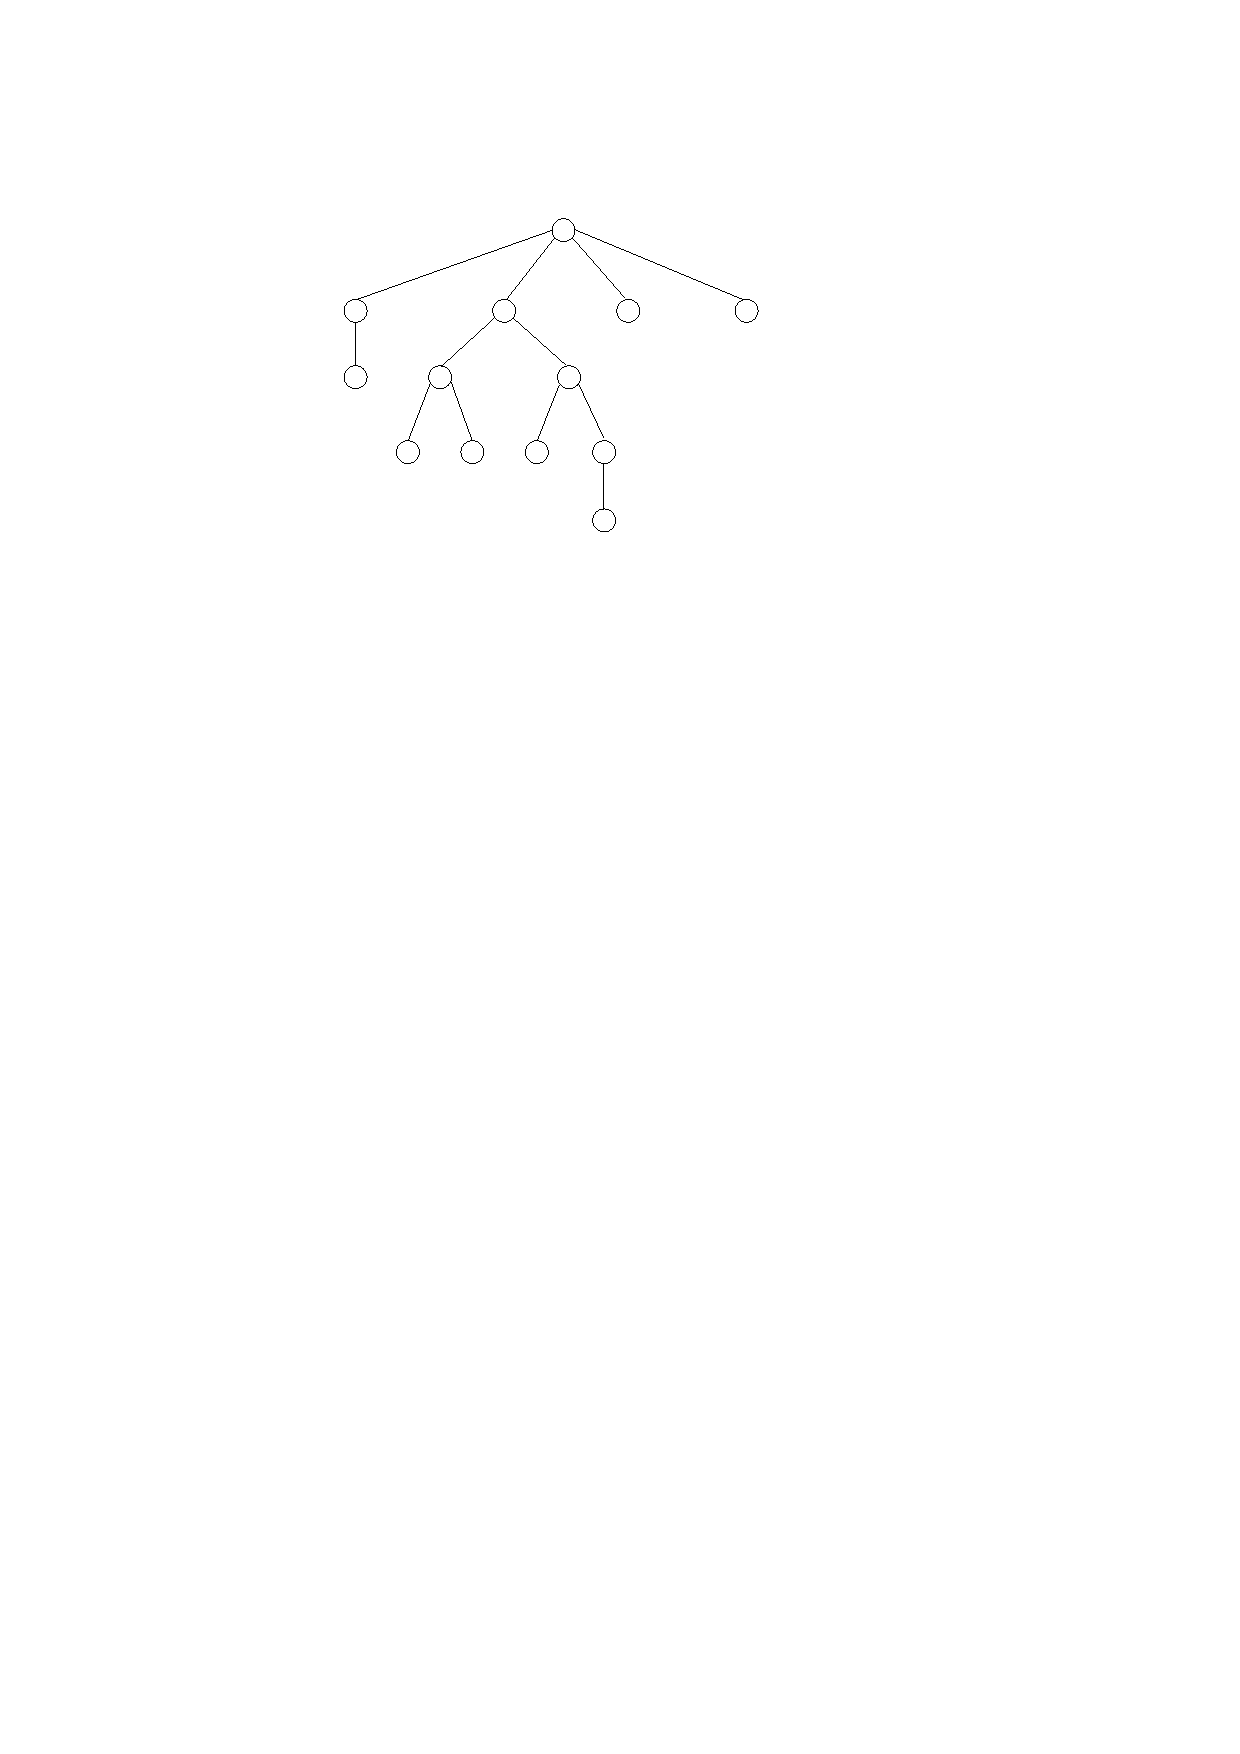
\includegraphics[scale=0.5]{images/bp.pdf}
\caption{An ordinal tree used as an example.}
\label{figure:bp}
\end{figure}

The fully function representation is not the first structure that makes use of balanced parentheses to represent trees. 
Munro and Raman~\cite{mr1997} first designed succinct representations of balanced parentheses, and they further used them to represent ordinal trees succinctly, by reducing a set of navigational operations over trees to operations over balanced parentheses. 
They only support a subset of the operations listed in table~\ref{tbl:operations}. 
To support more operations, researchers designed more auxiliary data structures~\cite{ly2008}. 
Thus, to support the operations in table~\ref{tbl:operations}, many auxiliary data structures are required, which make the overall data structure overtly complex in both theory and practice. 
The main novelty of Navarro and Sadakane's work~\cite{Navarro:2014:FFS:2620785.2601073} lies in their key strategy of reducing a large set of operations over trees and balanced parentheses to a small set of primitive operations. 
To define these operations, they treated $P$ as a bit vector, by storing a $1$ bit for each opening parenthesis, and a $0$ bit for a closing parenthesis. 
Let $g(\cdot)$ be a function on $[0,1]$. Then, they defined the following primitive operations:

\begin{myitemize}
\item $\sumop(P,g,i,j)\triangleq \sum_{k=i}^jg(P[k])$
\item $\fwdsearch(P,g,i,d)\triangleq \min\{j | j \ge i, \sumop(P,g,i,j) = d\}$
\item $\bwdsearch(P,g,i,d)\triangleq \max\{j | j \le i, \sumop(P,g,j,i) = d\}$
\item $\rmq(P,g,i,j)\triangleq \min\{\sumop(P,g,i,k)| i\le k\le j\}$
\item $\RMQ(P,g,i,j)\triangleq \max\{\sumop(P,g,i,k)| i\le k\le j\}$
\item $\rmqi(P,g,i,j)\triangleq \argmin_{k\in[i,j]}\{\sumop(P,g,i,k)\}$
\item $\RMQi(P,g,i,j)\triangleq \argmax_{k\in[i,j]}\{\sumop(P,g,i,k)\}$
\end{myitemize}

Navarro and Sadakane defined three functions on $[0,1]$: function $\pi$ such that $\pi(1) = 1$ and $\pi(0) = -1$, function $\phi$ such that $\phi(1) = 1$ and $\phi(0) = 0$, and function $\psi$ such that $\psi(1) = 0$ and $\psi(0) = 1$. 
Most of the operations in Table~\ref{tbl:operations} can then be supported using the primitive operations when setting $g(\cdot)$ to be $\pi$, $\phi$ and $\psi$. For example, $\findclose(i)$ can be computed using $\fwdsearch(P,\pi,i,0)$. 
Thus it suffices to support these primitive operations when $g(\cdot) = \pi$, $\phi$ or $\psi$, and a few  navigational operations in trees that can not supported by these primitive operations, which are $\degree$, $\child$, $\childrank$ and the four operations related to leaf nodes in table~\ref{tbl:operations}. 
To support these operations, a simple data structure called \emph{Range Min-Max tree} ({\tt RMMT}) was designed, supporting operations in logarithmic time when used to represent the entire sequence $P$. 
Then, to achieve constant-time support for operations, $P$ is further partitioned into chunks, each of which is represented by a {\tt RMMT}, which can support operations inside a chunk in constant time when the size of each chunk is small enough. Additional data structures are further constructed to support operations in constant time over the entire sequence $P$. 
% for trees of small size, which is further used to design a representation of large trees. 
%, which can support operations in logarthimic time if used to represent the entire sequence $P$. 
%Then, to achieve constant-time support for operations, $P$ is further partitioned into chuncks, each of which is represented by a {\tt RMTT}, and additional data structures are further constructed. 

\subsubsection{The Range Min-Max Tree}

Let $w$ denote the number of bits in a word. The range min-max tree ({\tt RMMT}) is designed to support the primitive operations for functions $\pi$, $\phi$ and $\psi$. %, when the tree represented has $n = w^c$ nodes for an arbitrary constant $c \ge 1$. % \footnote{Navarro and Sadakane~\cite{Navarro:2014:FFS:2620785.2601073} initially defined a {\tt RMMT} for a tree of polylogarthmic size, which is used as a building block for their solution that achieves constant-time support for operations. They mentioned that, when using this structure for the entire tree, the operations can only be supported in logarithmic time, but the structure is simple and practical, which was the variant implemented and tested in \cite{ACNSalenex10}. As we perform experimental studies on the parallel construction of a {\tt RMMT}, here we directly define it for the entire tree.}.
We first describe how to construct a {\tt RMMT} using the function $\pi$, and later we will show how this can be easily augmented to support the operations for the other two functions. 
Recall that $T$ denotes the input tree on $n$ nodes, and $P$ denotes its balance parenthesis sequence of length $2n$, where $P[i] = 1$ iff the $i$th parenthesis is an opening parenthesis. 
The {\em excess} value at position $i$ of $P$ is defined as $\sumop(P,\pi,0,i) = \sum_{k=0}^{i} \pi(P[k])$. 
Let $E$ be a conceptual array in which $E[i]$ stores the excess value at $P[i]$. 

To introduce the {\tt RMMT}, we first partition $P[1..2n]$ into disjoint chunks of size $s$. We will set a value for $s$ later, and for now, the only restriction is that $s \le w/2$. 
For simplicity, we assume that the length of $P$ is divisible by $s$. 
Each chunk is a leaf of the {\tt RMMT}. The {\tt RMMT} is then defined as a complete $k$-ary tree on these leaves, and we will discuss the choices of the values of $k$ later. %, where $k = \Theta(w/(c\lg w))$. 
The following four conceptual arrays, each of length $2n / s$, are defined: $e$, storing the excess value at the last position in each chunk, $m$, storing the minimum excess value inside
each chunk, $M$, storing the maximum excess value inside each
chunk, and $n^*$, storing the number of occurrences of the minimum
value in each chunk. 
Each internal node, $u$, of the {\tt RMMT} also stores in $e[u]$/$m[u]$/$M[u]$ the last/miniumum/maximum of the $e$/$m$/$M$ values stored in its children, and in $n^*[u]$ the total number of times $m[u]$ appears in the chucks corresponding to all the leaf descendants of $u$ in the {\tt RMMT}. 
For the values stored for each internal node and each leaf of the {\tt RMMT}, see Figure~\ref{fig:RangeMinMaxTree} for an example. 
As the {\tt RMMT} is a complete tree, we do not store its structure explicitly. 
Instead, we can simply store the $e$/$m$/$M$/$n^*$ values of its (internal and leaf) nodes in four arrays $e'$/$m'$/$M'$/$n'$, like a heap. 

\begin{figure}[ht]
  \centering
  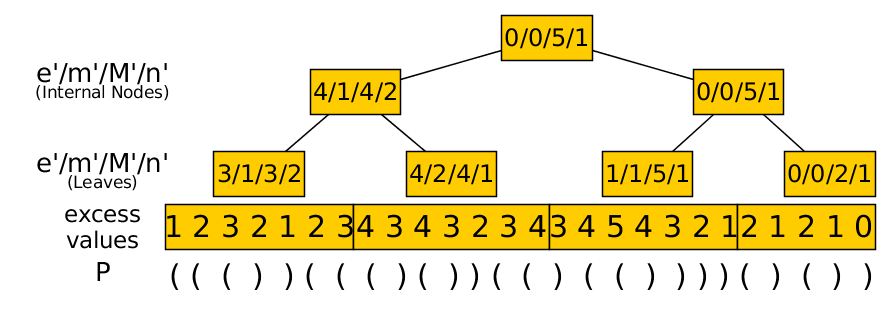
\includegraphics[scale=0.18]{./images/Range-min-max-tree.png}
  \caption{Range min-max tree}
  \label{fig:RangeMinMaxTree} 
\end{figure}

Combined with a standard succinct data structure technique called {\em table lookup}, a {\tt RMMT} can support the primitive operations for $\pi$, as well as $\degree$, $\child$ and $\childrank$. 
Take the support for $\fwdsearch(P,\pi,i,d)$ for example. 
We first check the chunk containing $P[i]$ to see if the answer is inside the same chunk. 
This can be done in constant time by constructing a universal lookup table whose content does not depend on $P$: For each possible bit vector of length $w/2$, and each of the $w/2$ position in the bit vector, we store the answer of $\fwdsearch(P,\pi,i,d)$ if it can be found inside this bit vector, or $-1$ otherwise. As there are $\sqrt{2^w}$ bit vectors of length $w/2$, this table uses $\sqrt{2^w}\poly(w)$ bits. 
If we find the  answer by performing a table lookup for the chunk containing $P[i]$, then we return. 
Otherwise, we search among the $m$ and $M$ values of the right siblings of the leaf node, $u$, corresponding to this chunk, to find the closest right sibling that contains the answer if the answer is within chunks represented by these siblings. 
If the $m$ and $M$ values (each using $\lceil\lg n\rceil$ bits) of the $k$ children of each internal node can be packed into $O(w)$ bits, i.e., $k \lg n = O(w)$, then we can again construct universal lookup tables for internal nodes to perform this step in constant time. 
We repeat this process until we find a right sibling, $v$, of an ancestor of $u$ whose corresponding substring of $P$ contains the answer. 
We then use a similar idea to descend down the tree starting from $v$ to look for the leaf descendant of $v$ containing the result. 
Thus we can support $\fwdsearch$ in $O(h)$ time where $h$ is the height of the {\tt RMMT}, provided that $k \lg n = O(w)$. 

To support the primitive operations for functions $\phi$ and $\psi$, we can define six arrays $e'_{\phi}$, $m'_{\phi}$, $M'_{\phi}$, $e'_{\psi}$, $m'_{\psi}$ and $M'_{\psi}$ which are similar to $e'$, $m'$ and $M'$ defined for $\pi$ ($n'$ is defined to support $\degree$, $\child$ and $\childrank$ only, and thus we need not define similar arrays for $\phi$ and $\psi$). 
We make use of the following three observations to avoid storing these six arrays explicitly: $\sumop(P, \phi, 0, i)$ and $\sumop(P, \psi, 0, i)$ are nondecreasing, $\sumop(P, \phi, 0, i) + \sumop(P, \psi, 0, i) = i$ and $\sumop(P, \phi, 0, i) - \sumop(P, \psi, 0, i) = \sumop(P, \pi, 0, i)$. 
Thus the each value in these six arrays can be computed in constant time without storing them explicitly. 
We just have to compute universal tables to support operations. 

To support $\leafrank$, $\leafselect$, $\lmostleaf$ and \linebreak $\rmostleaf$, we define a conceptual bit vector $P_1[1..2n]$ in which $P_1[i] = 1$ iff $P[i] = 1$ and $P[i+1] = 0$. 
Hence each $1$ bit in $P_1$ corresponds to a leaf node. 
The support for these operations are then reduced to the support for $\rankop$ and $\selop$ operations on $P_1$ defined as follows: $\rankop(P_1, i)$ returns the number of $1$s in $P_1[1..i]$, and $\selop(P_1, i)$ returns the position of the $i$th occurrence of $1$ in $P_1$. 
For example, we have $\leafrank = \rankop(P_1, i)$. 
The $\rankop$ and $\selop$ operations can be further reduced to the support of $\sumop$ and $\fwdsearch$ for the function $\phi$ on $P_1$, which can be supported using another range min-max tree. 
As any $O(w)$ bits in the sequence $P_1$ can be computed from $P$ in constant time using table lookup, $P_1$ itself need not be stored explicitly, and the cost of storing the information for the internal nodes of this range min-max tree is dominated by the space usage of the range min-max tree for $P$. 

To analyze the space cost, we observe that if we store $P$, $e'$, $m'$, $M'$ and $n'$ explicitly in a straightforward manner, the space cost would be $2n + \frac{k}{k-1} \cdot \frac{n}{s} \cdot \lg n$. 
Navarro and Sadakane commented that if we choose $s = w/2$ and $k = w / \lg n$, we will have a simple structure supporting all the operations in Table~\ref{tbl:operations} in $O(\lg n)$ time. 
However, when the trees are so large that $w = \Theta(\lg n)$, $e'$, $m'$, $M'$ and $n'$ would occupy $O(n)$ bits, and then the overall space is more than a typical succinct tree representation which would use $2n+o(n)$ bits. 
Here we comment that to reduce the overall space cost to $2n+o(n)$ bits, we can set $s = \lceil w\lg n\rceil$ and $k = 2$. With these parameters, looking for a potential answer to a query within a chunk would require $O(\lg n)$ table lookups, and as the height of the tree is $O(\lg n)$, operators can be supported in $O(\lg n)$ time. Note that since the tree is binary when $k = 2$, universal tables are not needed for internal nodes. Thus we have the following lemma:

\begin{lemma}\label{lem:lg}
An ordinal tree and its balanced parenthesis sequence can be represented using range min-max trees in $2n + o(n)$ bits, where $n$ is the number of nodes in the tree, to support the operations in Table~\ref{tbl:operations} in $O(\lg n)$ time. 
\end{lemma}

The data structure presented by Lemma~\ref{lem:lg} is practical, and previous experimental studies~\cite{ACNSalenex10} also chose to implement practical versions of RMMT that support operations in $O(\lg n)$ time. 
Navarro and Sadakane, however, initially designed RMMT in order to use it as a building block in their solution that represents trees succinctly to support operations in constant time. 
They choose a parameter $B = \Theta(\frac{w}{c\lg w})$, and construct a {\tt RMMT} for trees on $(B^c)/2$ nodes, where $c > 3/2$ is an arbitrary constant. 
Note that the length of the parenthesis sequence $P$ is now a power of $B$. 
They set $s = k = B$. 
Instead of storing $P$, $e'$, $m'$, $M'$ and $n'$ explicitly, they reduce the space cost by encoding them using the {\em aB-tree}~\cite{Patrascu:2008:SUC:1470582.1470670}. 
When constructed to store $P$, $e'$, $m'$, $M'$ and $n'$, an aB-tree stores $B$ consecutive elements of $P$ in each leaf, and the aB-tree is a complete $B$-ary tree. 
Thus the height of the tree is $c$, the time required to support operations in Table~\ref{tbl:operations} is $O(c) = O(1)$, and the space usage is $2n+2$ bits only. 
Note that universal tables are still required, but if we construct them for all possible bit vectors of length $B$, then their space costs are reduced to $\sqrt{2^w}$ bits. 

\subsubsection{Representing Large Trees}

To support operations in constant time for trees of arbitrary sizes, Navarro and Sadakane partition $P$ into {\em blocks} of length $w^c$. 
Each block may not necessarily store a balanced sequence, but it can still be represented using a {\tt RMMT} in $w^c + 2$ bits.  
The universal tables constructed for different blocks store the same content, so one set of these tables are sufficient. 
The overall space of storing the RMMT's of all these blocks and one set of universal tables is thus $2n + O(n/w^c) + \sqrt{2^w}$ bits. 

2d min-heap

weighted ancestor

rmq

rest